% Options for packages loaded elsewhere
\PassOptionsToPackage{unicode}{hyperref}
\PassOptionsToPackage{hyphens}{url}
%
\documentclass[
  Letterpaper,
]{scrbook}

\usepackage{amsmath,amssymb}
\usepackage{iftex}
\ifPDFTeX
  \usepackage[T1]{fontenc}
  \usepackage[utf8]{inputenc}
  \usepackage{textcomp} % provide euro and other symbols
\else % if luatex or xetex
  \usepackage{unicode-math}
  \defaultfontfeatures{Scale=MatchLowercase}
  \defaultfontfeatures[\rmfamily]{Ligatures=TeX,Scale=1}
\fi
\usepackage{lmodern}
\ifPDFTeX\else  
    % xetex/luatex font selection
    \setmainfont[]{Georgia}
\fi
% Use upquote if available, for straight quotes in verbatim environments
\IfFileExists{upquote.sty}{\usepackage{upquote}}{}
\IfFileExists{microtype.sty}{% use microtype if available
  \usepackage[]{microtype}
  \UseMicrotypeSet[protrusion]{basicmath} % disable protrusion for tt fonts
}{}
\makeatletter
\@ifundefined{KOMAClassName}{% if non-KOMA class
  \IfFileExists{parskip.sty}{%
    \usepackage{parskip}
  }{% else
    \setlength{\parindent}{0pt}
    \setlength{\parskip}{6pt plus 2pt minus 1pt}}
}{% if KOMA class
  \KOMAoptions{parskip=half}}
\makeatother
\usepackage{xcolor}
\usepackage[paperwidth=6in,paperheight=9in]{geometry}
\setlength{\emergencystretch}{3em} % prevent overfull lines
\setcounter{secnumdepth}{5}
% Make \paragraph and \subparagraph free-standing
\makeatletter
\ifx\paragraph\undefined\else
  \let\oldparagraph\paragraph
  \renewcommand{\paragraph}{
    \@ifstar
      \xxxParagraphStar
      \xxxParagraphNoStar
  }
  \newcommand{\xxxParagraphStar}[1]{\oldparagraph*{#1}\mbox{}}
  \newcommand{\xxxParagraphNoStar}[1]{\oldparagraph{#1}\mbox{}}
\fi
\ifx\subparagraph\undefined\else
  \let\oldsubparagraph\subparagraph
  \renewcommand{\subparagraph}{
    \@ifstar
      \xxxSubParagraphStar
      \xxxSubParagraphNoStar
  }
  \newcommand{\xxxSubParagraphStar}[1]{\oldsubparagraph*{#1}\mbox{}}
  \newcommand{\xxxSubParagraphNoStar}[1]{\oldsubparagraph{#1}\mbox{}}
\fi
\makeatother


\providecommand{\tightlist}{%
  \setlength{\itemsep}{0pt}\setlength{\parskip}{0pt}}\usepackage{longtable,booktabs,array}
\usepackage{calc} % for calculating minipage widths
% Correct order of tables after \paragraph or \subparagraph
\usepackage{etoolbox}
\makeatletter
\patchcmd\longtable{\par}{\if@noskipsec\mbox{}\fi\par}{}{}
\makeatother
% Allow footnotes in longtable head/foot
\IfFileExists{footnotehyper.sty}{\usepackage{footnotehyper}}{\usepackage{footnote}}
\makesavenoteenv{longtable}
\usepackage{graphicx}
\makeatletter
\newsavebox\pandoc@box
\newcommand*\pandocbounded[1]{% scales image to fit in text height/width
  \sbox\pandoc@box{#1}%
  \Gscale@div\@tempa{\textheight}{\dimexpr\ht\pandoc@box+\dp\pandoc@box\relax}%
  \Gscale@div\@tempb{\linewidth}{\wd\pandoc@box}%
  \ifdim\@tempb\p@<\@tempa\p@\let\@tempa\@tempb\fi% select the smaller of both
  \ifdim\@tempa\p@<\p@\scalebox{\@tempa}{\usebox\pandoc@box}%
  \else\usebox{\pandoc@box}%
  \fi%
}
% Set default figure placement to htbp
\def\fps@figure{htbp}
\makeatother
% definitions for citeproc citations
\NewDocumentCommand\citeproctext{}{}
\NewDocumentCommand\citeproc{mm}{%
  \begingroup\def\citeproctext{#2}\cite{#1}\endgroup}
\makeatletter
 % allow citations to break across lines
 \let\@cite@ofmt\@firstofone
 % avoid brackets around text for \cite:
 \def\@biblabel#1{}
 \def\@cite#1#2{{#1\if@tempswa , #2\fi}}
\makeatother
\newlength{\cslhangindent}
\setlength{\cslhangindent}{1.5em}
\newlength{\csllabelwidth}
\setlength{\csllabelwidth}{3em}
\newenvironment{CSLReferences}[2] % #1 hanging-indent, #2 entry-spacing
 {\begin{list}{}{%
  \setlength{\itemindent}{0pt}
  \setlength{\leftmargin}{0pt}
  \setlength{\parsep}{0pt}
  % turn on hanging indent if param 1 is 1
  \ifodd #1
   \setlength{\leftmargin}{\cslhangindent}
   \setlength{\itemindent}{-1\cslhangindent}
  \fi
  % set entry spacing
  \setlength{\itemsep}{#2\baselineskip}}}
 {\end{list}}
\usepackage{calc}
\newcommand{\CSLBlock}[1]{\hfill\break\parbox[t]{\linewidth}{\strut\ignorespaces#1\strut}}
\newcommand{\CSLLeftMargin}[1]{\parbox[t]{\csllabelwidth}{\strut#1\strut}}
\newcommand{\CSLRightInline}[1]{\parbox[t]{\linewidth - \csllabelwidth}{\strut#1\strut}}
\newcommand{\CSLIndent}[1]{\hspace{\cslhangindent}#1}

\usepackage{makeidx}
\makeindex
\raggedbottom
\makeatletter
\@ifpackageloaded{bookmark}{}{\usepackage{bookmark}}
\makeatother
\makeatletter
\@ifpackageloaded{caption}{}{\usepackage{caption}}
\AtBeginDocument{%
\ifdefined\contentsname
  \renewcommand*\contentsname{Table of contents}
\else
  \newcommand\contentsname{Table of contents}
\fi
\ifdefined\listfigurename
  \renewcommand*\listfigurename{List of Figures}
\else
  \newcommand\listfigurename{List of Figures}
\fi
\ifdefined\listtablename
  \renewcommand*\listtablename{List of Tables}
\else
  \newcommand\listtablename{List of Tables}
\fi
\ifdefined\figurename
  \renewcommand*\figurename{Figure}
\else
  \newcommand\figurename{Figure}
\fi
\ifdefined\tablename
  \renewcommand*\tablename{Table}
\else
  \newcommand\tablename{Table}
\fi
}
\@ifpackageloaded{float}{}{\usepackage{float}}
\floatstyle{ruled}
\@ifundefined{c@chapter}{\newfloat{codelisting}{h}{lop}}{\newfloat{codelisting}{h}{lop}[chapter]}
\floatname{codelisting}{Listing}
\newcommand*\listoflistings{\listof{codelisting}{List of Listings}}
\makeatother
\makeatletter
\makeatother
\makeatletter
\@ifpackageloaded{caption}{}{\usepackage{caption}}
\@ifpackageloaded{subcaption}{}{\usepackage{subcaption}}
\makeatother

\usepackage{bookmark}

\IfFileExists{xurl.sty}{\usepackage{xurl}}{} % add URL line breaks if available
\urlstyle{same} % disable monospaced font for URLs
\hypersetup{
  pdftitle={The Vagus Advantage},
  pdfauthor={Dr.~Ray Zhang and Richard Sprague},
  hidelinks,
  pdfcreator={LaTeX via pandoc}}


\title{The Vagus Advantage}
\usepackage{etoolbox}
\makeatletter
\providecommand{\subtitle}[1]{% add subtitle to \maketitle
  \apptocmd{\@title}{\par {\large #1 \par}}{}{}
}
\makeatother
\subtitle{Harnessing Neural Stimulation for Modern Wellness}
\author{Dr.~Ray Zhang and Richard Sprague}
\date{2025-05-14}

\begin{document}
\frontmatter
\maketitle

\renewcommand*\contentsname{Table of contents}
{
\setcounter{tocdepth}{2}
\tableofcontents
}

\mainmatter
\bookmarksetup{startatroot}

\chapter*{Preface}\label{preface}
\addcontentsline{toc}{chapter}{Preface}

\markboth{Preface}{Preface}

The book you hold in your hands represents the culmination of thousands
of hours of research, clinical observation, and technological
development by a dedicated team committed to advancing our understanding
of neural regulation and its practical applications. ``The Vagus
Advantage'' is not merely an academic exercise but a bridge between
cutting-edge neuroscience and everyday wellness---a guide to harnessing
the remarkable potential of vagus nerve stimulation in our increasingly
demanding world.

Our journey began with a simple yet profound observation: the human
nervous system, particularly the vagus nerve, holds untapped potential
for improving how we manage stress, enhance cognitive performance, and
recover from the demands of modern life. This ``neural highway'' that
connects brain and body offers a gateway to influencing our most
essential physiological functions---from heart rate and digestion to
attention and emotional regulation.

This work stands on the shoulders of pioneers in neuroscience who have
illuminated the intricate mechanisms of neural function. We owe a
particular debt of gratitude to Dr.~Robert Desimone, Director of the
McGovern Institute and Doris and Don Berkey Professor of Brain and
Cognitive Sciences, whose groundbreaking research on attention
mechanisms has fundamentally shaped our understanding of how the brain
processes information. As Dr.~Desimone eloquently observes:

\begin{quote}
``Our brains are constantly bombarded with sensory information. The
ability to distinguish relevant information from irrelevant distractions
is a critical skill, one that is impaired in many brain disorders. By
studying the visual system of humans and animals, our research has shown
that when we attend to something specific, neurons in certain brain
regions fire in unison -- like a chorus rising above the noise --
allowing the relevant information to be `heard' more efficiently by
other regions of the brain.''
\end{quote}

This powerful metaphor of neural synchronization---a ``chorus rising
above the noise''---captures beautifully what vagus nerve stimulation
offers: a means to orchestrate our neural activity more harmoniously,
enhancing signal over noise in both brain and body. The technology we
explore in this book draws inspiration from this understanding, offering
a non-invasive approach to influencing these natural neural rhythms.

We have written this book for a diverse audience: healthcare
professionals seeking additional tools for patient care, researchers
interested in the intersection of neuroscience and wellness technology,
and individuals looking to take a more active role in managing their
mental and physical wellbeing. Whether you approach this subject with
scientific curiosity, professional interest, or personal motivation, we
believe you'll find valuable insights in the pages that follow.

Throughout this book, we maintain a commitment to scientific integrity
while acknowledging that we stand at the frontier of an evolving field.
We present the established research alongside emerging findings, always
distinguishing between what is known with certainty and what remains
promising but preliminary. Our goal is not to oversell the technology's
capabilities but to present a balanced assessment of its current
applications and future potential.

The journey from laboratory discovery to practical, everyday technology
is rarely straightforward. As you'll discover in these pages, vagus
nerve stimulation has traveled a fascinating path from clinical
treatment for specific medical conditions to a broader tool for wellness
optimization. We invite you to explore this journey with us and consider
how these advances might enhance your professional practice or personal
wellbeing.

With gratitude for your interest in this emerging field,

\emph{The Authors}\\
May 2025

\bookmarksetup{startatroot}

\chapter*{Introduction}\label{introduction}
\addcontentsline{toc}{chapter}{Introduction}

\markboth{Introduction}{Introduction}

\bookmarksetup{startatroot}

\chapter{The Vagus Nerve: Anatomy and Function of Your Body's Neural
Highway}\label{the-vagus-nerve-anatomy-and-function-of-your-bodys-neural-highway}

\bookmarksetup{startatroot}

\chapter{The Science of Neural Regulation: How VNS Affects Brain and
Body}\label{the-science-of-neural-regulation-how-vns-affects-brain-and-body}

\bookmarksetup{startatroot}

\chapter{From Medical Intervention to Wellness Tool: The Evolution of
VNS
Technology}\label{from-medical-intervention-to-wellness-tool-the-evolution-of-vns-technology}

\bookmarksetup{startatroot}

\chapter{From Medical Intervention to Wellness Tool: The Evolution of
VNS
Technology}\label{from-medical-intervention-to-wellness-tool-the-evolution-of-vns-technology-1}

\bookmarksetup{startatroot}

\chapter{Managing Stress and Anxiety: VNS as a Neurological
Intervention}\label{managing-stress-and-anxiety-vns-as-a-neurological-intervention}

\bookmarksetup{startatroot}

\chapter{Managing Stress and Anxiety: VNS as a Neurological
Intervention}\label{managing-stress-and-anxiety-vns-as-a-neurological-intervention-1}

\bookmarksetup{startatroot}

\chapter{The Cognitive Edge: VNS for Focus, Attention and Mental
Performance}\label{the-cognitive-edge-vns-for-focus-attention-and-mental-performance}

\bookmarksetup{startatroot}

\chapter{The Cognitive Edge: VNS for Focus, Attention and Mental
Performance}\label{the-cognitive-edge-vns-for-focus-attention-and-mental-performance-1}

\bookmarksetup{startatroot}

\chapter{Better Rest: Applications of VNS for Sleep Quality and
Recovery}\label{better-rest-applications-of-vns-for-sleep-quality-and-recovery}

\bookmarksetup{startatroot}

\chapter{Better Rest: Applications of VNS for Sleep Quality and
Recovery}\label{better-rest-applications-of-vns-for-sleep-quality-and-recovery-1}

\bookmarksetup{startatroot}

\chapter{The Hardware Landscape: Comparing VNS Device
Technologies}\label{the-hardware-landscape-comparing-vns-device-technologies}

\bookmarksetup{startatroot}

\chapter{The Hardware Landscape: Comparing VNS Device
Technologies}\label{the-hardware-landscape-comparing-vns-device-technologies-1}

\bookmarksetup{startatroot}

\chapter{Optimal Stimulation: Parameters, Protocols and
Personalization}\label{optimal-stimulation-parameters-protocols-and-personalization}

\bookmarksetup{startatroot}

\chapter{Optimal Stimulation: Parameters, Protocols and
Personalization}\label{optimal-stimulation-parameters-protocols-and-personalization-1}

\bookmarksetup{startatroot}

\chapter{Integrating VNS into Daily Life: Practical Applications and Use
Cases}\label{integrating-vns-into-daily-life-practical-applications-and-use-cases}

Here is our first headphone

\begin{figure}[H]

{\centering \pandocbounded{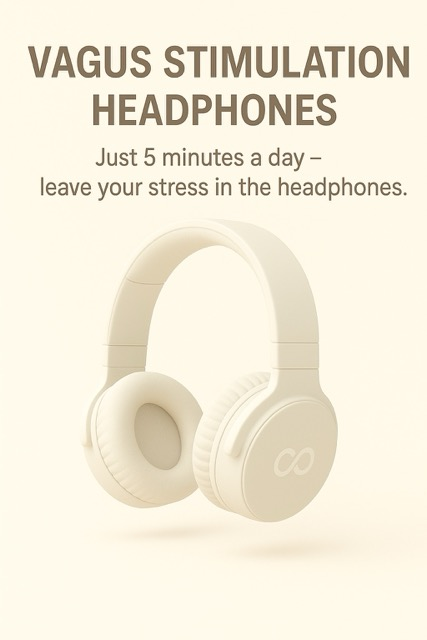
\includegraphics[keepaspectratio]{_resources/images/VNSImage Medium.jpeg}}

}

\caption{The best headphones for VNS}

\end{figure}%

\bookmarksetup{startatroot}

\chapter{The Future of Neural Wellness: Closed-Loop Systems and
AI-Enhanced
VNS}\label{the-future-of-neural-wellness-closed-loop-systems-and-ai-enhanced-vns}

\bookmarksetup{startatroot}

\chapter{The Future of Neural Wellness: Closed-Loop Systems and
AI-Enhanced
VNS}\label{the-future-of-neural-wellness-closed-loop-systems-and-ai-enhanced-vns-1}

\bookmarksetup{startatroot}

\chapter{Summary and Conclusions}\label{summary-and-conclusions}

\bookmarksetup{startatroot}

\chapter{Summary and Conclusions}\label{summary-and-conclusions-1}

\bookmarksetup{startatroot}

\chapter{References}\label{references}

\bookmarksetup{startatroot}

\chapter*{References}\label{references-1}
\addcontentsline{toc}{chapter}{References}

\markboth{References}{References}

\phantomsection\label{refs}
\begin{CSLReferences}{1}{0}
\bibitem[\citeproctext]{ref-addorisioInvestigationalTreatmentRheumatoid2019}
Addorisio, Meghan E., Gavin H. Imperato, Alex F. De Vos, Steve Forti,
Richard S. Goldstein, Valentin A. Pavlov, Tom Van Der Poll, et al. 2019.
{``Investigational Treatment of Rheumatoid Arthritis with a Vibrotactile
Device Applied to the External Ear.''} \emph{Bioelectronic Medicine} 5
(1): 4. \url{https://doi.org/10.1186/s42234-019-0020-4}.

\bibitem[\citeproctext]{ref-alkhawajahImpactAutonomicNervous2024}
Alkhawajah, Hani A., Ali M. Y. Alshami, and Ali M. Albarrati. 2024.
{``The {Impact} of {Autonomic Nervous System Modulation} on {Heart Rate
Variability} and {Musculoskeletal Manifestations} in {Chronic Neck
Pain}: {A Double-Blind Randomized Clinical Trial}.''} \emph{Journal of
Clinical Medicine} 14 (1): 153.
\url{https://doi.org/10.3390/jcm14010153}.

\bibitem[\citeproctext]{ref-badranNeurophysiologicEffectsTranscutaneous2018}
Badran, Bashar W., Logan T. Dowdle, Oliver J. Mithoefer, Nicholas T.
LaBate, James Coatsworth, Joshua C. Brown, William H. DeVries,
Christopher W. Austelle, Lisa M. McTeague, and Mark S. George. 2018.
{``Neurophysiologic Effects of Transcutaneous Auricular Vagus Nerve
Stimulation ({taVNS}) via Electrical Stimulation of the Tragus: {A}
Concurrent {taVNS}/{fMRI} Study and Review.''} \emph{Brain Stimulation}
11 (3): 492--500. \url{https://doi.org/10.1016/j.brs.2017.12.009}.

\bibitem[\citeproctext]{ref-bolzTechnicalAspectsFuture2022}
Bolz, Armin, and Lars-Oliver Bolz. 2022. {``Technical Aspects and Future
Approaches in Transcutaneous Vagus Nerve Stimulation ({tVNS}).''}
\emph{Autonomic Neuroscience} 239 (May): 102956.
\url{https://doi.org/10.1016/j.autneu.2022.102956}.

\bibitem[\citeproctext]{ref-bremnerApplicationNoninvasiveVagal2020}
Bremner, James Douglas, Nil Z. Gurel, Matthew T. Wittbrodt, Mobashir H.
Shandhi, Mark H. Rapaport, Jonathon A. Nye, Bradley D. Pearce, et al.
2020. {``Application of {Noninvasive Vagal Nerve Stimulation} to
{Stress-Related Psychiatric Disorders}.''} \emph{Journal of Personalized
Medicine} 10 (3): 119. \url{https://doi.org/10.3390/jpm10030119}.

\bibitem[\citeproctext]{ref-bublSeeingGrayWhen2010}
Bubl, Emanuel, Elena Kern, Dieter Ebert, Michael Bach, and Ludger
Tebartz Van Elst. 2010. {``Seeing {Gray When Feeling Blue}? {Depression
Can Be Measured} in the {Eye} of the {Diseased}.''} \emph{Biological
Psychiatry} 68 (2): 205--8.
\url{https://doi.org/10.1016/j.biopsych.2010.02.009}.

\bibitem[\citeproctext]{ref-canliAmygdalaReactivityEmotional2005}
Canli, Turhan, Rebecca E. Cooney, Philippe Goldin, Maulik Shah, Heidi
Sivers, Moriah E. Thomason, Susan Whitfield-Gabrieli, John D. E.
Gabrieli, and Ian H. Gotlib. 2005. {``Amygdala Reactivity to Emotional
Faces Predicts Improvement in Major Depression.''} \emph{NeuroReport} 16
(12): 1267--70.
\url{https://doi.org/10.1097/01.wnr.0000174407.09515.cc}.

\bibitem[\citeproctext]{ref-canliBrainActivationEmotional2004}
Canli, Turhan, Heidi Sivers, Moriah E. Thomason, Susan
Whitfield-Gabrieli, John D. E. Gabrieli, and Ian H. Gotlib. 2004.
{``Brain Activation to Emotional Words in Depressed Vs Healthy
Subjects:''} \emph{NeuroReport} 15 (17): 2585--88.
\url{https://doi.org/10.1097/00001756-200412030-00005}.

\bibitem[\citeproctext]{ref-caoAccuracyAssessmentOura2022}
Cao, Rui, Iman Azimi, Fatemeh Sarhaddi, Hannakaisa Niela-Vilen, Anna
Axelin, Pasi Liljeberg, and Amir M Rahmani. 2022. {``Accuracy
{Assessment} of {Oura Ring Nocturnal Heart Rate} and {Heart Rate
Variability} in {Comparison With Electrocardiography} in {Time} and
{Frequency Domains}: {Comprehensive Analysis}.''} \emph{Journal of
Medical Internet Research} 24 (1): e27487.
\url{https://doi.org/10.2196/27487}.

\bibitem[\citeproctext]{ref-capilupiVagusNerveStimulation2020}
Capilupi, Michael J., Samantha M. Kerath, and Lance B. Becker. 2020.
{``Vagus {Nerve Stimulation} and the {Cardiovascular System}.''}
\emph{Cold Spring Harbor Perspectives in Medicine} 10 (2): a034173.
\url{https://doi.org/10.1101/cshperspect.a034173}.

\bibitem[\citeproctext]{ref-chaiFunctionalStructuralBrain2015}
Chai, Xiaoqian J., Dina Hirshfeld-Becker, Joseph Biederman, Mai Uchida,
Oliver Doehrmann, Julia A. Leonard, John Salvatore, et al. 2015.
{``Functional and Structural Brain Correlates of Risk for Major
Depression in Children with Familial Depression.''} \emph{NeuroImage:
Clinical} 8: 398--407. \url{https://doi.org/10.1016/j.nicl.2015.05.004}.

\bibitem[\citeproctext]{ref-constableRetinalElectrophysiologyCentral2023}
Constable, Paul A., Jeremiah K. H. Lim, and Dorothy A. Thompson. 2023.
{``Retinal Electrophysiology in Central Nervous System Disorders. {A}
Review of Human and Mouse Studies.''} \emph{Frontiers in Neuroscience}
17 (August): 1215097. \url{https://doi.org/10.3389/fnins.2023.1215097}.

\bibitem[\citeproctext]{ref-danthineElectroencephalogramSynchronizationMeasure2024}
Danthine, Venethia, Lise Cottin, Alexandre Berger, Enrique Ignacio
Germany Morrison, Giulia Liberati, Susana Ferrao Santos, Jean Delbeke,
Antoine Nonclercq, and Riëm El Tahry. 2024. {``Electroencephalogram
Synchronization Measure as a Predictive Biomarker of {Vagus} Nerve
Stimulation Response in Refractory Epilepsy: {A} Retrospective Study.''}
Edited by Ayataka Fujimoto. \emph{PLOS ONE} 19 (6): e0304115.
\url{https://doi.org/10.1371/journal.pone.0304115}.

\bibitem[\citeproctext]{ref-dingClassifyingMajorDepression2019}
Ding, Xinfang, Xinxin Yue, Rui Zheng, Cheng Bi, Dai Li, and Guizhong
Yao. 2019. {``Classifying Major Depression Patients and Healthy Controls
Using {EEG}, Eye Tracking and Galvanic Skin Response Data.''}
\emph{Journal of Affective Disorders} 251 (May): 156--61.
\url{https://doi.org/10.1016/j.jad.2019.03.058}.

\bibitem[\citeproctext]{ref-erturkComparisonAcuteEffects2025}
Ertürk, Çağıl, and Ali Veysel Özden. 2025. {``Comparison of the {Acute
Effects} of {Auricular Vagus Nerve Stimulation} and {Deep Breathing
Exercise} on the {Autonomic Nervous System Activity} and {Biomechanical
Properties} of the {Muscle} in {Healthy People}.''} \emph{Journal of
Clinical Medicine} 14 (4): 1046.
\url{https://doi.org/10.3390/jcm14041046}.

\bibitem[\citeproctext]{ref-fangPreoperativeHeartRate2021}
Fang, Xi, Hong-Yun Liu, Zhi-Yan Wang, Zhao Yang, Tung-Yang Cheng,
Chun-Hua Hu, Hong-Wei Hao, et al. 2021. {``Preoperative {Heart Rate
Variability During Sleep Predicts Vagus Nerve Stimulation Outcome
Better} in {Patients With Drug-Resistant Epilepsy}.''} \emph{Frontiers
in Neurology} 12 (July): 691328.
\url{https://doi.org/10.3389/fneur.2021.691328}.

\bibitem[\citeproctext]{ref-farmerInternationalConsensusBased2021}
Farmer, Adam D., Adam Strzelczyk, Alessandra Finisguerra, Alexander V.
Gourine, Alireza Gharabaghi, Alkomiet Hasan, Andreas M. Burger, et al.
2021. {``International {Consensus Based Review} and {Recommendations}
for {Minimum Reporting Standards} in {Research} on {Transcutaneous Vagus
Nerve Stimulation} ({Version} 2020).''} \emph{Frontiers in Human
Neuroscience} 14 (March): 568051.
\url{https://doi.org/10.3389/fnhum.2020.568051}.

\bibitem[\citeproctext]{ref-farrandVagusNerveStimulation2023}
Farrand, Ariana, Vincent Jacquemet, Ryan Verner, Misty Owens, and Eric
Beaumont. 2023. {``Vagus Nerve Stimulation Parameters Evoke Differential
Neuronal Responses in the Locus Coeruleus.''} \emph{Physiological
Reports} 11 (5): e15633. \url{https://doi.org/10.14814/phy2.15633}.

\bibitem[\citeproctext]{ref-forteEarYourHeart2022}
Forte, Giuseppe, Francesca Favieri, Erik Leemhuis, Maria Luisa De
Martino, Anna Maria Giannini, Luigi De Gennaro, Maria Casagrande, and
Mariella Pazzaglia. 2022. {``Ear Your Heart: Transcutaneous Auricular
Vagus Nerve Stimulation on Heart Rate Variability in Healthy Young
Participants.''} \emph{PeerJ} 10 (November): e14447.
\url{https://doi.org/10.7717/peerj.14447}.

\bibitem[\citeproctext]{ref-galinPredictivePotentialHeart2024}
Galin, Shir, and Hanna Keren. 2024. {``The {Predictive Potential} of
{Heart Rate Variability} for {Depression}.''} \emph{Neuroscience} 546
(May): 88--103.
\url{https://doi.org/10.1016/j.neuroscience.2024.03.013}.

\bibitem[\citeproctext]{ref-gencEffectsVagalNerve2024}
Genç, Ahmet, Firdevs Ezgi Uçan Tokuç, and Meltem Korucuk. 2024.
{``Effects of Vagal Nerve Stimulation Parameters on Heart Rate
Variability in Epilepsy Patients.''} \emph{Frontiers in Neurology} 15
(October): 1490887. \url{https://doi.org/10.3389/fneur.2024.1490887}.

\bibitem[\citeproctext]{ref-gotlibSubgenualAnteriorCingulate2005}
Gotlib, Ian H., Heidi Sivers, John D. E. Gabrieli, Susan
Whitfield-Gabrieli, Philippe Goldin, Kelly L. Minor, and Turhan Canli.
2005. {``Subgenual Anterior Cingulate Activation to Valenced Emotional
Stimuli in Major Depression.''} \emph{NeuroReport} 16 (16): 1731--34.
\url{https://doi.org/10.1097/01.wnr.0000183901.70030.82}.

\bibitem[\citeproctext]{ref-hartmannHeartRateVariability2019}
Hartmann, Ralf, Frank M. Schmidt, Christian Sander, and Ulrich Hegerl.
2019. {``Heart {Rate Variability} as {Indicator} of {Clinical State} in
{Depression}.''} \emph{Frontiers in Psychiatry} 9 (January): 735.
\url{https://doi.org/10.3389/fpsyt.2018.00735}.

\bibitem[\citeproctext]{ref-jensenModulatingHeartRate2022}
Jensen, Mette Kjeldsgaard, Sally Søgaard Andersen, Stine Søgaard
Andersen, Caroline Hundborg Liboriussen, Salome Kristensen, and Mads
Jochumsen. 2022. {``Modulating {Heart Rate Variability} Through {Deep
Breathing Exercises} and {Transcutaneous Auricular Vagus Nerve
Stimulation}: {A Study} in {Healthy Participants} and in {Patients} with
{Rheumatoid Arthritis} or {Systemic Lupus Erythematosus}.''}
\emph{Sensors} 22 (20): 7884. \url{https://doi.org/10.3390/s22207884}.

\bibitem[\citeproctext]{ref-jiaoEffectTranscutaneousVagus2020}
Jiao, Yue, Xiao Guo, Man Luo, Suxia Li, Aihua Liu, Yufeng Zhao, Bin
Zhao, et al. 2020. {``Effect of {Transcutaneous Vagus Nerve Stimulation}
at {Auricular Concha} for {Insomnia}: {A Randomized Clinical Trial}.''}
Edited by Francesca Mancianti. \emph{Evidence-Based Complementary and
Alternative Medicine} 2020 (1): 6049891.
\url{https://doi.org/10.1155/2020/6049891}.

\bibitem[\citeproctext]{ref-kimEffectsVagusNerve2022}
Kim, Jeong Sik, Do Eon Lee, Hyoeun Bae, Joo Yeon Song, Kwang Ik Yang,
and Seung Bong Hong. 2022. {``Effects of {Vagus Nerve Stimulation} on
{Sleep-Disordered Breathing}, {Daytime Sleepiness}, and {Sleep Quality}
in {Patients With Drug-Resistant Epilepsy}.''} \emph{Journal of Clinical
Neurology} 18 (3): 315. \url{https://doi.org/10.3988/jcn.2022.18.3.315}.

\bibitem[\citeproctext]{ref-kochMetaanalysisHeartRate2019}
Koch, Celine, Marcel Wilhelm, Stefan Salzmann, Winfried Rief, and Frank
Euteneuer. 2019. {``A Meta-Analysis of Heart Rate Variability in Major
Depression.''} \emph{Psychological Medicine} 49 (12): 1948--57.
\url{https://doi.org/10.1017/S0033291719001351}.

\bibitem[\citeproctext]{ref-kurdiIntroducingOpenAffective2017}
Kurdi, Benedek, Shayn Lozano, and Mahzarin R. Banaji. 2017.
{``Introducing the {Open Affective Standardized Image Set} ({OASIS}).''}
\emph{Behavior Research Methods} 49 (2): 457--70.
\url{https://doi.org/10.3758/s13428-016-0715-3}.

\bibitem[\citeproctext]{ref-maPreventiveNoninvasiveVagal2024}
Ma, Sai-Nan, Xiao-Hong Liu, and Wei-Song Cai. 2024. {``Preventive
Noninvasive Vagal Nerve Stimulation Reduces Insufficient Sleep-Induced
Depression by Improving the Autonomic Nervous System.''}
\emph{Biomedicine \& Pharmacotherapy} 173 (April): 116344.
\url{https://doi.org/10.1016/j.biopha.2024.116344}.

\bibitem[\citeproctext]{ref-masonHeartRateVariability2024}
Mason, Federico, Anna Scarabello, Lisa Taruffi, Elena Pasini, Giovanna
Calandra-Buonaura, Luca Vignatelli, and Francesca Bisulli. 2024.
{``Heart {Rate Variability} as a {Tool} for {Seizure Prediction}: {A
Scoping Review}.''} \emph{Journal of Clinical Medicine} 13 (3): 747.
\url{https://doi.org/10.3390/jcm13030747}.

\bibitem[\citeproctext]{ref-mitseaDigitallyAssistedMindfulness2023}
Mitsea, Eleni, Athanasios Drigas, and Charalabos Skianis. 2023.
{``Digitally {Assisted Mindfulness} in {Training Self-Regulation Skills}
for {Sustainable Mental Health}: {A Systematic Review}.''}
\emph{Behavioral Sciences} 13 (12): 1008.
\url{https://doi.org/10.3390/bs13121008}.

\bibitem[\citeproctext]{ref-nickelAnalysisSkinCorneal2024}
Nickel, Kathrin, Ludger Tebartz Van Elst, Malina Beringer, Dominique
Endres, Kimon Runge, Simon Maier, Sebastian Küchlin, et al. 2024.
{``Analysis of Skin and Corneal Fiber Electrodes for Electroretinogram
Assessments in Patients with Major Depressive Disorder.''}
\emph{Frontiers in Neuroscience} 18 (November): 1501149.
\url{https://doi.org/10.3389/fnins.2024.1501149}.

\bibitem[\citeproctext]{ref-ogradyValidityAppleWatch2024}
O'Grady, Ben, Rory Lambe, Maximus Baldwin, Tara Acheson, and Cailbhe
Doherty. 2024. {``The {Validity} of {Apple Watch Series} 9 and {Ultra} 2
for {Serial Measurements} of {Heart Rate Variability} and {Resting Heart
Rate}.''} \emph{Sensors} 24 (19): 6220.
\url{https://doi.org/10.3390/s24196220}.

\bibitem[\citeproctext]{ref-pervazDoesTranscutaneousAuricular2025}
Pervaz, Ipek, Lilly Thurn, Cecilia Vezzani, Luisa Kaluza, Anne Kühnel,
and Nils B. Kroemer. 2025. {``Does Transcutaneous Auricular Vagus Nerve
Stimulation Alter Pupil Dilation? {A} Living {Bayesian}
Meta-Analysis.''} \emph{Brain Stimulation} 18 (2): 148--57.
\url{https://doi.org/10.1016/j.brs.2025.01.022}.

\bibitem[\citeproctext]{ref-raileUsefulnessChatGPTPsychotherapists2024}
Raile, Paolo. 2024. {``The Usefulness of {ChatGPT} for Psychotherapists
and Patients.''} \emph{Humanities and Social Sciences Communications} 11
(1): 47. \url{https://doi.org/10.1057/s41599-023-02567-0}.

\bibitem[\citeproctext]{ref-redgraveSafetyTolerabilityTranscutaneous2018}
Redgrave, J., D. Day, H. Leung, P. J. Laud, A. Ali, R. Lindert, and A.
Majid. 2018. {``Safety and Tolerability of {Transcutaneous Vagus Nerve}
Stimulation in Humans; a Systematic Review.''} \emph{Brain Stimulation}
11 (6): 1225--38. \url{https://doi.org/10.1016/j.brs.2018.08.010}.

\bibitem[\citeproctext]{ref-rembadoCorticalResponsesVagus2021}
Rembado, Irene, Weiguo Song, David K Su, Ariel Levari, Larry E Shupe,
Steve Perlmutter, Eberhard Fetz, and Stavros Zanos. 2021. {``Cortical
{Responses} to {Vagus Nerve Stimulation Are Modulated} by {Brain State}
in {Nonhuman Primates}.''} \emph{Cerebral Cortex} 31 (12): 5289--5307.
\url{https://doi.org/10.1093/cercor/bhab158}.

\bibitem[\citeproctext]{ref-rongEffectTranscutaneousAuricular2016}
Rong, Peijing, Jun Liu, Liping Wang, Rupeng Liu, Jiliang Fang, Jingjun
Zhao, Yufeng Zhao, et al. 2016. {``Effect of Transcutaneous Auricular
Vagus Nerve Stimulation on Major Depressive Disorder: {A} Nonrandomized
Controlled Pilot Study.''} \emph{Journal of Affective Disorders} 195
(May): 172--79. \url{https://doi.org/10.1016/j.jad.2016.02.031}.

\bibitem[\citeproctext]{ref-sethEffectsVagusNerve2024}
Seth, Jayant, R. Grace Couper, Jorge G. Burneo, and Ana Suller Marti.
2024. {``Effects of Vagus Nerve Stimulation on the Quality of Sleep and
Sleep Apnea in Patients with Drug-Resistant Epilepsy: {A} Systematic
Review.''} \emph{Epilepsia} 65 (1): 73--83.
\url{https://doi.org/10.1111/epi.17811}.

\bibitem[\citeproctext]{ref-shaperoNeuralMarkersDepression2019}
Shapero, Benjamin G., Xiaoqian J. Chai, Mark Vangel, Joseph Biederman,
Christian S. Hoover, Susan Whitfield-Gabrieli, John D. E. Gabrieli, and
Dina R. Hirshfeld-Becker. 2019. {``Neural Markers of Depression Risk
Predict the Onset of Depression.''} \emph{Psychiatry Research:
Neuroimaging} 285 (March): 31--39.
\url{https://doi.org/10.1016/j.pscychresns.2019.01.006}.

\bibitem[\citeproctext]{ref-sharonTranscutaneousVagusNerve2021}
Sharon, Omer, Firas Fahoum, and Yuval Nir. 2021. {``Transcutaneous
{Vagus Nerve Stimulation} in {Humans Induces Pupil Dilation} and
{Attenuates Alpha Oscillations}.''} \emph{The Journal of Neuroscience}
41 (2): 320--30. \url{https://doi.org/10.1523/JNEUROSCI.1361-20.2020}.

\bibitem[\citeproctext]{ref-siddalsItHappenedBe2024}
Siddals, Steven, John Torous, and Astrid Coxon. 2024. {``{`{It} Happened
to Be the Perfect Thing'}: Experiences of Generative {AI} Chatbots for
Mental Health.''} \emph{Npj Mental Health Research} 3 (1): 48.
\url{https://doi.org/10.1038/s44184-024-00097-4}.

\bibitem[\citeproctext]{ref-toschiCausalInfluenceBrainstem2023}
Toschi, Nicola, Andrea Duggento, Riccardo Barbieri, Ronald G. Garcia,
Harrison P. Fisher, Norman W. Kettner, Vitaly Napadow, and Roberta
Sclocco. 2023. {``Causal Influence of Brainstem Response to
Transcutaneous Vagus Nerve Stimulation on Cardiovagal Outflow.''}
\emph{Brain Stimulation} 16 (6): 1557--65.
\url{https://doi.org/10.1016/j.brs.2023.10.007}.

\bibitem[\citeproctext]{ref-wangAdvancesVNSEfficiency2024}
Wang, Wendi, Rui Li, Chuangtao Li, Qimin Liang, and Xiaolin Gao. 2024.
{``Advances in {VNS} Efficiency and Mechanisms of Action on Cognitive
Functions.''} \emph{Frontiers in Physiology} 15 (October): 1452490.
\url{https://doi.org/10.3389/fphys.2024.1452490}.

\bibitem[\citeproctext]{ref-winterVagusNerveStimulation2024}
Winter, Yaroslav, Katharina Sandner, Claudio L. A. Bassetti, Martin
Glaser, Dumitru Ciolac, Andreas Ziebart, Ali Karakoyun, et al. 2024.
{``Vagus Nerve Stimulation for the Treatment of Narcolepsy.''}
\emph{Brain Stimulation} 17 (1): 83--88.
\url{https://doi.org/10.1016/j.brs.2024.01.002}.

\bibitem[\citeproctext]{ref-woodhamHomebasedTranscranialDirect2025}
Woodham, Rachel D., Sudhakar Selvaraj, Nahed Lajmi, Harriet Hobday,
Gabrielle Sheehan, Ali-Reza Ghazi-Noori, Peter J. Lagerberg, et al.
2025. {``Home-Based Transcranial Direct Current Stimulation Treatment
for Major Depressive Disorder: A Fully Remote Phase 2 Randomized
Sham-Controlled Trial.''} \emph{Nature Medicine} 31 (1): 87--95.
\url{https://doi.org/10.1038/s41591-024-03305-y}.

\bibitem[\citeproctext]{ref-wuTranscutaneousVagusNerve2022}
Wu, Yating, Lu Song, Xian Wang, Ning Li, Shuqin Zhan, Peijing Rong,
Yuping Wang, and Aihua Liu. 2022. {``Transcutaneous {Vagus Nerve
Stimulation Could Improve} the {Effective Rate} on the {Quality} of
{Sleep} in the {Treatment} of {Primary Insomnia}: {A Randomized Control
Trial}.''} \emph{Brain Sciences} 12 (10): 1296.
\url{https://doi.org/10.3390/brainsci12101296}.

\bibitem[\citeproctext]{ref-xuEffectivenessSafetyTranscutaneous2025}
Xu, Zheng Yan Ran, Jia Jia Fang, Xiao Qin Fan, Long Long Xu, Gui Fang
Jin, Mei Hua Lei, Yu Fei Wang, et al. 2025. {``Effectiveness and Safety
of Transcutaneous Auricular Vagus Nerve Stimulation for Depression in
Patients with Epilepsy.''} \emph{Epilepsy \& Behavior} 163 (February):
110226. \url{https://doi.org/10.1016/j.yebeh.2024.110226}.

\bibitem[\citeproctext]{ref-yakuninaOptimizationTranscutaneousVagus2017}
Yakunina, Natalia, Sam Soo Kim, and Eui-Cheol Nam. 2017. {``Optimization
of {Transcutaneous Vagus Nerve Stimulation Using Functional MRI}.''}
\emph{Neuromodulation: Technology at the Neural Interface} 20 (3):
290--300. \url{https://doi.org/10.1111/ner.12541}.

\bibitem[\citeproctext]{ref-yangTranscutaneousAuricularVagus2024}
Yang, Ting, Yunhuo Cai, Xingling Li, Lianqiang Fang, and Hantong Hu.
2024. {``Is Transcutaneous Auricular Vagus Nerve Stimulation Effective
and Safe for Primary Insomnia? {A PRISMA-compliant} Protocol for a
Systematic Review and Meta-Analysis.''} Edited by Yung-Hsiang Chen.
\emph{PLOS ONE} 19 (11): e0313101.
\url{https://doi.org/10.1371/journal.pone.0313101}.

\bibitem[\citeproctext]{ref-zhangEffectsTranscutaneousAuricular2021}
Zhang, Shuai, Jia-Kai He, Hong Meng, Bin Zhao, Ya-Nan Zhao, Yu Wang,
Shao-Yuan Li, et al. 2021. {``Effects of Transcutaneous Auricular Vagus
Nerve Stimulation on Brain Functional Connectivity of Medial Prefrontal
Cortex in Patients with Primary Insomnia.''} \emph{The Anatomical
Record} 304 (11): 2426--35. \url{https://doi.org/10.1002/ar.24785}.

\end{CSLReferences}


\backmatter

\printindex


\end{document}
